\documentclass[12pt,letterpaper,titlepage]{article}

\usepackage{fontspec}
\defaultfontfeatures{Mapping=tex-text}
\usepackage{xunicode}
\usepackage{xltxtra}
\usepackage{amsmath}
\usepackage{pdfpages}
\usepackage{amsfonts}
\usepackage{bbold}
\usepackage{amssymb}
\setcounter{secnumdepth}{0}
\usepackage{nameref}
\usepackage{enumitem}
\usepackage{environ}
\usepackage{pgfplots}

\showboxdepth=\maxdimen
\showboxbreadth=\maxdimen


\usepackage{paracol}
\usepackage{wrapfig}
\globalcounter{table}
\globalcounter{figure}
\usepackage{graphicx}
\usepackage[left=1in,right=1in,top=1in,bottom=1in]{geometry}
\graphicspath{{img/}}

\author{Jacob Abel}
\title{	Design \& Simulate 3 Ex1.4
	\\\large ECE2204 CRN:82929
}

\setlength{\parskip}{0.5em}

\begin{document}
\maketitle
\begin{raggedright}

\section{Problem 3.4.a.1: }
\subsection{Design}

Consider silicon at $T = 300 K$ with a diffusion current density of $J_n = 200 A/cm^2$. Assume that the electron concentration varies linearly over the distance from $x = 0$ to $x = 7 \mu m$ from $n_{lower} = 10^{13} cm^{−3}$ to some unknown upper electron concentration $n_{upper}$. Assume $D_n = 32 cm^2/s$ and that the value of the elementary charge is $\mathbb{e} = 1.6\cdot 10^{-19} C$. Calculate the upper electron concentration $n_{upper}$.


\begin{equation}\scalebox{1.25}{
$
J_n = e D_n \frac{\Delta n}{\Delta x} \implies n_{upper} = \frac{J_n\times \Delta x}{\mathbb{e} D_n} + n_{lower}
$
}
\end{equation}
\begin{equation}\scalebox{1.25}{
$
n_{upper} = \frac{200 A/cm^2 \times 7\mu m}{1.6\times 10^{-19} C \times 32cm^2/s} + 10^{13} cm^{−3} = 2.735 \times 10^{16} cm^{-3} 
$
}
\end{equation}
	
The upper electron concentration is $n_{upper} = 2.735 \times 10^{16} cm^{-3}$.
	
\subsection{Validation}

\begin{center}
Mathematica Implementation (accurate with $< 1`\%$ deviation from design result)
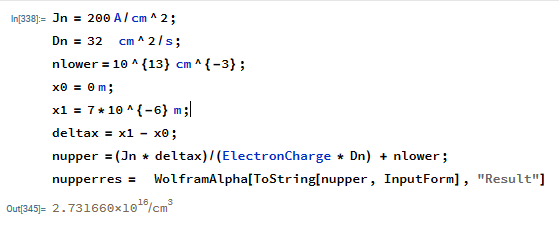
\includegraphics[width=.75\textwidth, height=\textheight, keepaspectratio=true]{ds1a}
$Err = \frac{|2.735-2.731|}{2.735} = 0.00146 = 0.146\%$
\end{center}

\begin{center}
LTSpice Implementation (equivalent within 4 significant figures)
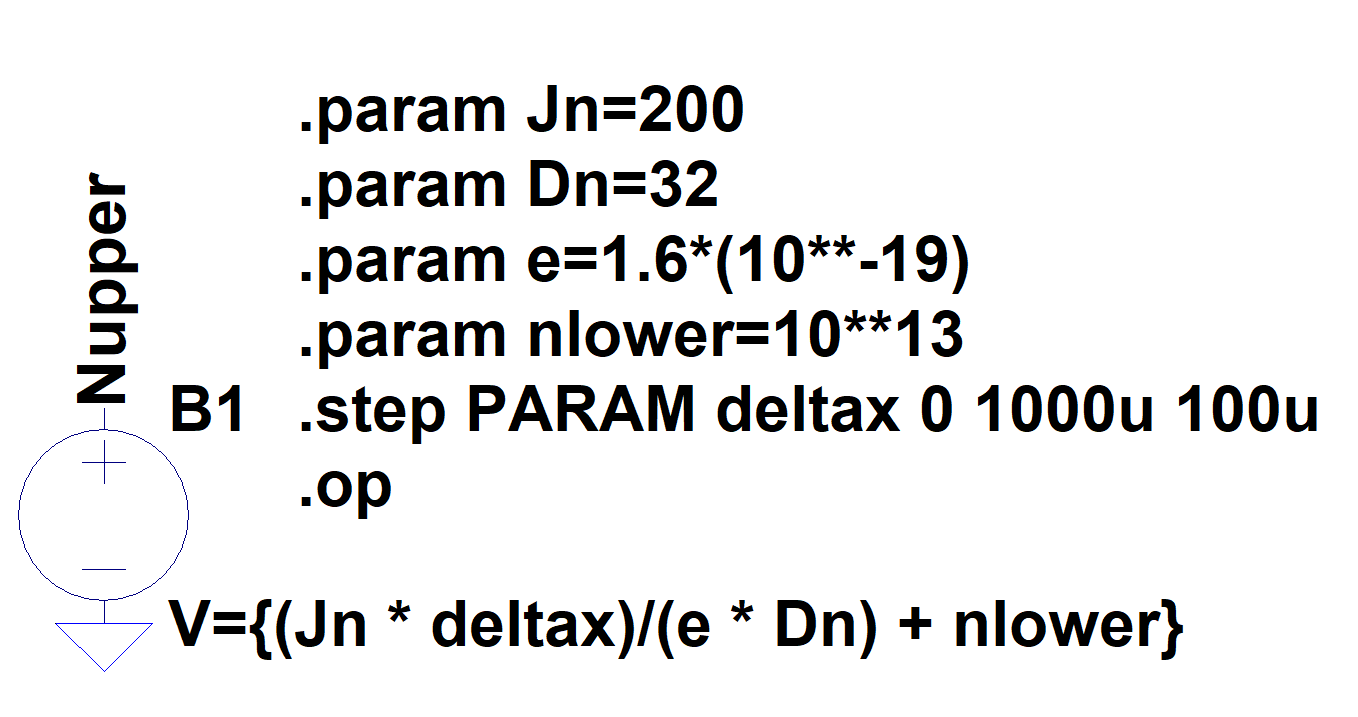
\includegraphics[width=.4\textwidth, height=\textheight, keepaspectratio=true]{ds1b}
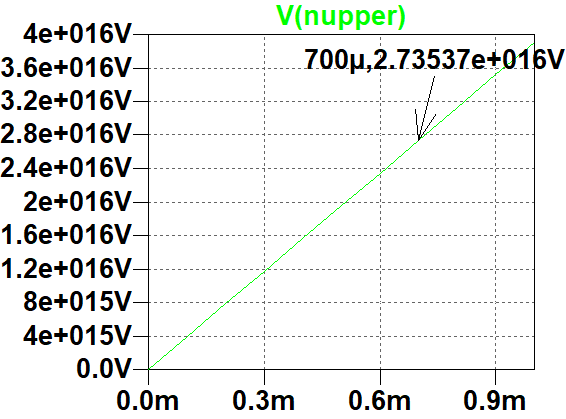
\includegraphics[width=.4\textwidth, height=\textheight, keepaspectratio=true]{ds1c}
\end{center}

\clearpage
\section{Problem 3.4.b.1: }
\subsection{Design}
The hole concentration in silicon is given by 

\begin{equation}\scalebox{1.25}{
$
p(x) = 10^3 + 10^{12} e^\frac{−x}{L_p}\quad x \geq 0
$
}
\end{equation}

The value of $L_p$ is $13\mu m$. The hole diffusion coefficient is $D_p = 66 cm^2/s$. Assume the value of the elementary charge is $\mathbb{e} = 1.6\cdot 10^{-19} C$. Determine the hole diffusion current density at $x = 23\mu m$.

\begin{equation}\scalebox{1.25}{
$
\frac{dp}{dx}p(x) = \frac{-10^{12}}{L_p} e^\frac{-x}{L_p}
$
}
\end{equation}

\begin{equation}\scalebox{1.25}{
$
J_p = -\mathbb{e} D_p \frac{dp}{dx} \implies J_p = \mathbb{e} D_p \frac{10^{12}}{L_p} e^\frac{-x}{L_p} \times cm^{-3}
$
}
\end{equation}

\begin{equation}\scalebox{1.25}{
$
J_p = \mathbb{e} \times 66 cm^2/s \times \frac{10^{12}}{13\mu m} e^\frac{-23\mu m}{13\mu m} \times cm^{-3}
	= 1.387 \times 10^{-3} A/cm^2
$
}
\end{equation}




The hole diffusion current density $J_p = 1.387 \times 10^{-3} A/cm^2$.

\subsection{Validation}

\begin{center}
LTSpice Implementation (accurate with $< 1\%$ deviation from design result)
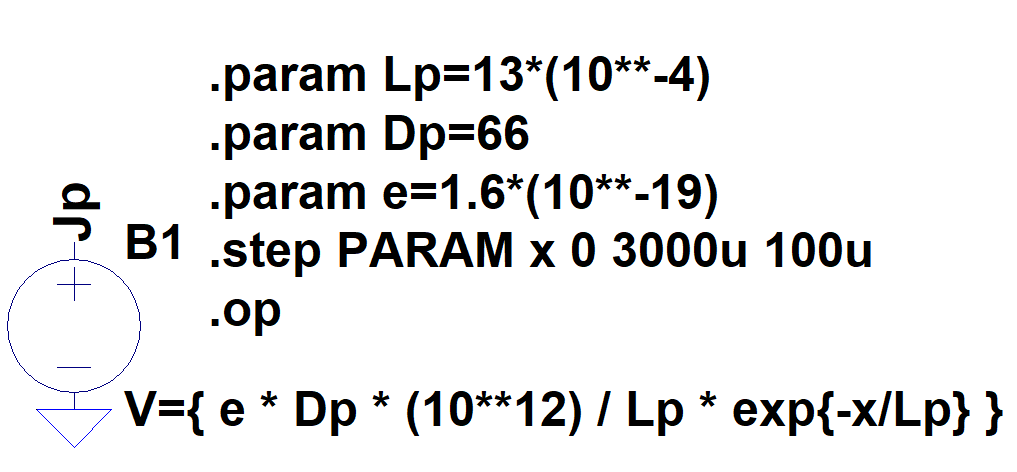
\includegraphics[width=.4\textwidth, height=\textheight, keepaspectratio=true]{ds2b}
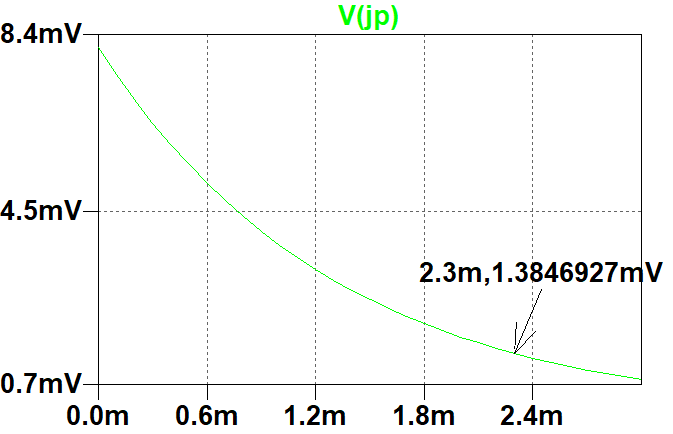
\includegraphics[width=.4\textwidth, height=\textheight, keepaspectratio=true]{ds2c}
$Err = \frac{|1.387-1.384|}{1.387} = 0.00216 = 0.216\%$
\end{center}

\textit{I have neither given nor received unauthorized assistance on this assignment.}


\end{raggedright}
\end{document}
